\documentclass[tikz,border=5pt]{standalone}
\usepackage{amssymb,amsmath}
\usetikzlibrary{calc}
\newcommand{\C}{\mathbb{C}}
\newcommand{\CP}{\mathbb{CP}}
\newcommand{\Res}{\operatorname{Res}}
\begin{document}
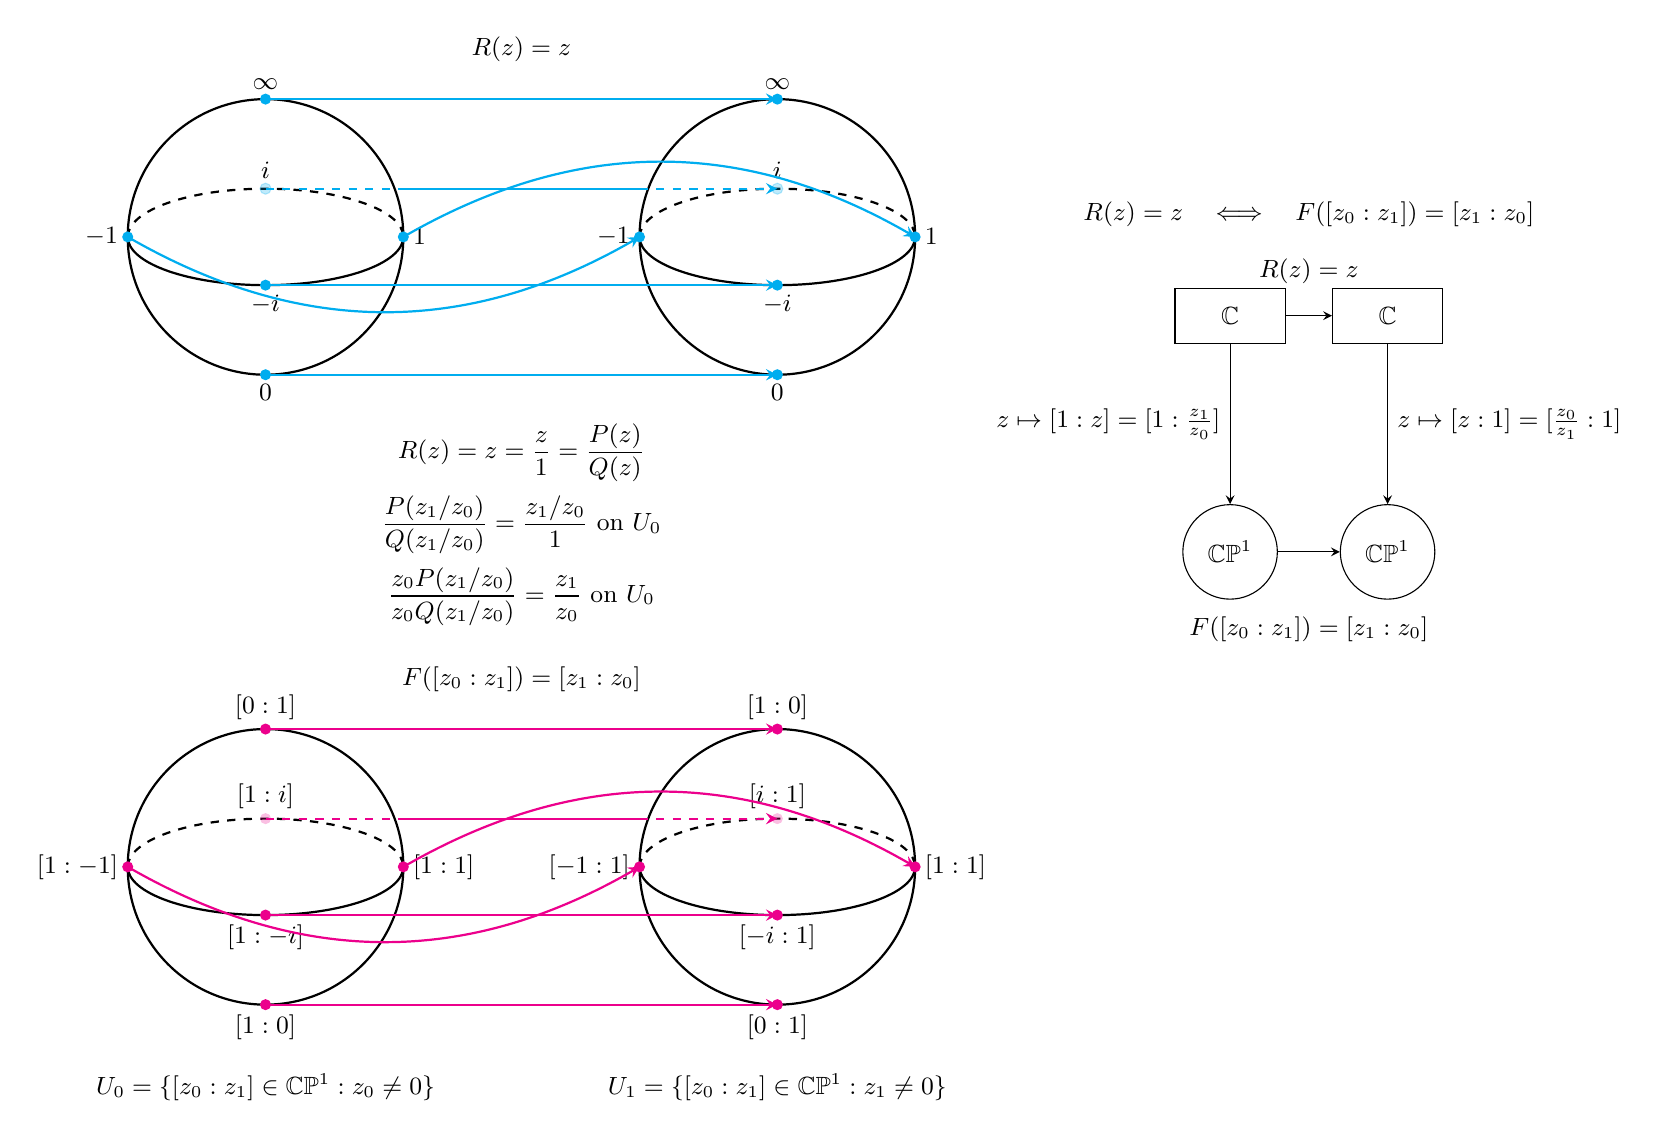
\begin{tikzpicture}[font=\small,>=stealth]
\tikzset{
	spoint/.style={circle,fill,inner sep=1.2pt},
	cp1/.style={circle,draw,minimum width=1.2cm},
	cplane/.style={rectangle,draw,minimum width=1.4cm,minimum height=0.7cm}
}
% Macro: draw a "3D-looking" sphere with 4 marked points
% Arguments: center x, center y, radius, name prefix
\newcommand{\SphereThreeD}[4]{%
% Main circle
\draw[thick] (#1,#2) circle (#3);
% Equator (back dashed, front solid)
\draw[thick] (#1-#3,#2) arc (180:360:#3 and 0.35*#3); % back
\draw[thick, dashed]        (#1-#3,#2) arc (180:0:#3 and 0.35*#3);   % front
% Points:
% N (∞), S (0), E (1), W (-1), I (i), MI (-i)
\coordinate (#4N)  at (#1,#2+#3);            % north pole: infinity
\coordinate (#4S)  at (#1,#2-#3);            % south pole: 0
\coordinate (#4E)  at (#1+#3,#2);            % east equator: 1
\coordinate (#4W)  at (#1-#3,#2);            % west equator: -1
\coordinate (#4I)  at (#1,#2+0.35*#3);       % upper meridian: i
\coordinate (#4MI) at (#1,#2-0.35*#3);       % lower meridian: -i
% Draw points
\fill[spoint, cyan] (#4N)  circle (2pt);
\fill[spoint, cyan] (#4S)  circle (2pt);
\fill[spoint, cyan] (#4E)  circle (2pt);
\fill[spoint, cyan] (#4W)  circle (2pt);
\draw[spoint, cyan, opacity=.25] (#4I)  circle (2pt);
\fill[spoint, cyan] (#4MI) circle (2pt);
% Labels
\node[above]      at (#4N)  {$\infty$};
\node[below]      at (#4S)  {$0$};
\node[right]      at (#4E)  {$1$};
\node[left]       at (#4W)  {$-1$};
\node[above] at (#4I)  {$i$};
\node[below] at (#4MI) {$-i$};
}
\newcommand{\SphereCPzChart}[4]{%
	% Main circle
	\draw[thick] (#1,#2) circle (#3);
	% Equator (back dashed, front solid)
	\draw[thick] (#1-#3,#2) arc (180:360:#3 and 0.35*#3); % back
	\draw[thick, dashed]        (#1-#3,#2) arc (180:0:#3 and 0.35*#3);   % front
	% Points:
	% N (∞), S (0), E (1), W (-1), I (i), MI (-i)
	\coordinate (#4N)  at (#1,#2+#3);            % north pole: infinity
	\coordinate (#4S)  at (#1,#2-#3);            % south pole: 0
	\coordinate (#4E)  at (#1+#3,#2);            % east equator: 1
	\coordinate (#4W)  at (#1-#3,#2);            % west equator: -1
	\coordinate (#4I)  at (#1,#2+0.35*#3);       % upper meridian: i
	\coordinate (#4MI) at (#1,#2-0.35*#3);       % lower meridian: -i
	% Draw points
	\fill[spoint,magenta] (#4N)  circle (2pt);
	\fill[spoint,magenta] (#4S)  circle (2pt);
	\fill[spoint,magenta] (#4E)  circle (2pt);
	\fill[spoint,magenta] (#4W)  circle (2pt);
	\fill[spoint,magenta, opacity=.25] (#4I)  circle (2pt);
	\fill[spoint,magenta] (#4MI) circle (2pt);
	% Labels
	\node[above]      at (#4N)  {$[0:1]$};
	\node[below]      at (#4S)  {$[1:0]$};
	\node[right]      at (#4E)  {$[1:1]$};
	\node[left]       at (#4W)  {$[1:-1]$};
	\node[above] at (#4I)  {$[1:i]$};
	\node[below] at (#4MI) {$[1:-i]$};
}
\newcommand{\SphereCPwChart}[4]{%
% Main circle
\draw[thick] (#1,#2) circle (#3);
% Equator (back dashed, front solid)
\draw[thick] (#1-#3,#2) arc (180:360:#3 and 0.35*#3); % back
\draw[thick, dashed]        (#1-#3,#2) arc (180:0:#3 and 0.35*#3);   % front
% Points:
% N (∞), S (0), E (1), W (-1), I (i), MI (-i)
\coordinate (#4N)  at (#1,#2+#3);            % north pole: infinity
\coordinate (#4S)  at (#1,#2-#3);            % south pole: 0
\coordinate (#4E)  at (#1+#3,#2);            % east equator: 1
\coordinate (#4W)  at (#1-#3,#2);            % west equator: -1
\coordinate (#4I)  at (#1,#2+0.35*#3);       % upper meridian: i
\coordinate (#4MI) at (#1,#2-0.35*#3);       % lower meridian: -i
% Draw points
\fill[spoint,magenta] (#4N)  circle (2pt);
\fill[spoint,magenta] (#4S)  circle (2pt);
\fill[spoint,magenta] (#4E)  circle (2pt);
\fill[spoint,magenta] (#4W)  circle (2pt);
\fill[spoint,magenta, opacity=.25] (#4I)  circle (2pt);
\fill[spoint,magenta] (#4MI) circle (2pt);
% Labels
\node[above]      at (#4N)  {$[1:0]$};
\node[below]      at (#4S)  {$[0:1]$};
\node[right]      at (#4E)  {$[1:1]$};
\node[left]       at (#4W)  {$[-1:1]$};
\node[above] at (#4I)  {$[i:1]$};
\node[below] at (#4MI) {$[-i:1]$};
}
%%%%%%%%%%%%%%%%%%%%%%%%%%%%%%%%%%%%%%%%%%%%%%%%%%%%%%%%%%%%
% Panel 1: R(z) = z  (identity)
%%%%%%%%%%%%%%%%%%%%%%%%%%%%%%%%%%%%%%%%%%%%%%%%%%%%%%%%%%%%
\begin{scope}[shift={(0,6)}]
\node[above] at (0,2.1) {$R(z)=z$};
	\node[below,align=center] at (0,-2.25) {
%		$R(z)=z\leftrightarrow F([z_0:z_1])=[z_1:z_0]$ \\ [12pt]
		$\displaystyle R(z)=z=\frac{z}{1}=\frac{P(z)}{Q(z)}$\\ [4pt]
		$\displaystyle \frac{P(z_1/z_0)}{Q(z_1/z_0)}=\frac{z_1/z_0}{1}$ on $U_0$\\ [4pt]
		$\displaystyle \frac{z_0P(z_1/z_0)}{z_0Q(z_1/z_0)}=\frac{z_1}{z_0}$ on $U_0$\\ [4pt]
%		$R(i)=i\leftrightarrow F([i:1])=[1:i]$\\ [4pt]
%		$R(-i)=-i\leftrightarrow F([-i:1])=[1:-i]$\\ [4pt]
%		$R(\infty)=\infty\leftrightarrow F([1:0])=[0:1]$
	};

% Left and right spheres
\SphereThreeD{-3.25}{0}{1.75}{A}
\SphereThreeD{ 3.25}{0}{1.75}{B}

% Straight arrows: each special point maps to itself
\draw[->,thick,cyan] (AN) to (BN);
\draw[->,thick,cyan] (AS) to (BS);
\draw[->,thick,cyan] (AE) to[bend left] (BE);
\draw[->,thick,cyan] (AW) to[bend right] (BW);
\draw[thick,cyan,dashed] (AI) to (-1.5,.6125);
\draw[thick,cyan] (-1.5,.6125) to (1.5,.6125);
\draw[->,thick,cyan,dashed] (1.5,.6125) to (3.25,.6125);
\draw[->,thick,cyan] (AMI) to (BMI);
\end{scope}
\begin{scope}[shift={(0,-2)}]
\node[above] at (0,2.1) {$F([z_0:z_1])=[z_1:z_0]$};
%\node[below,align=center] at (0,-4) {
%	$R(0)=0\leftrightarrow F([1:0])=[0:1]$\\ [4pt]
%	$R(1)=1\leftrightarrow F([1:1])=[1:1]$\\ [4pt]
%	$R(-1)=1\leftrightarrow F([1:i])=[i:1]$\\ [4pt]
%	$R(i)=i\leftrightarrow F([1:-1])=[-1:1]$\\ [4pt]
%	$R(-i)=-i\leftrightarrow F([1:-i])=[-i:1]$\\ [4pt]
%	$R(\infty)=\infty\leftrightarrow F([0:1])=[1:0]$
%};
% Left and right spheres
\SphereCPzChart{-3.25}{0}{1.75}{A}
\SphereCPwChart{ 3.25}{0}{1.75}{B}
\node[below] at (-3.25,-2.5) {$U_0=\{[z_0:z_1]\in\CP^1:z_0\neq 0\}$};
\node[below] at (3.25,-2.5) {$U_1=\{[z_0:z_1]\in\CP^1:z_1\neq 0\}$};
% Straight arrows: each special point maps to itself
\draw[->,thick,magenta] (AN) to (BN);
\draw[->,thick,magenta] (AS) to (BS);
\draw[->,thick,magenta] (AE) to[bend left] (BE);
\draw[->,thick,magenta] (AW) to[bend right] (BW);
\draw[thick,magenta,dashed] (AI) to (-1.5,.6125);
\draw[thick,magenta] (-1.5,.6125) to (1.5,.6125);
\draw[->,thick,magenta,dashed] (1.5,.6125) to (3.25,.6125);
\draw[->,thick,magenta] (AMI) to (BMI);
\end{scope}


%========================================
% Diagram 1: R(z) = z  <->  F([z0:z1]) = [z1:z0]
% (as written by the user)
%========================================
\begin{scope}[shift={(10,4)}]
% Title
\node[above] at (0,2.0) {$R(z) = z \quad\Longleftrightarrow\quad
	F([z_0:z_1]) = [z_1:z_0]$};
% C -> C
\node[cplane] (CL1) at (-1,1) {$\C$};
\node[cplane] (CR1) at ( 1,1) {$\C$};
\draw[->] (CL1) -- (CR1)
node[midway,above=8] {$R(z)=z$};
% CP^1 -> CP^1
\node[cp1] (CP1L1) at (-1,-2) {$\CP^1$};
\node[cp1] (CP1R1) at ( 1,-2) {$\CP^1$};
\draw[->] (CP1L1) -- (CP1R1)
node[midway,below=20] {$F([z_0:z_1])=[z_1:z_0]$};

% Vertical arrows: affine chart z = z0/z1
\draw[->] (CL1) -- (CP1L1)
node[midway,left] {\(\displaystyle z\mapsto[1:z]=[1:\tfrac{z_1}{z_0}]\)};
\draw[->] (CR1) -- (CP1R1)
node[midway,right] {\(\displaystyle z\mapsto[z:1]=[\tfrac{z_0}{z_1}:1]\)};
\end{scope}

%%%%%%%%%%%%%%%%%%%%%%%%%%%%%%%%%%%%%%%%%%%%%%%%%%%%%%%%%%%%%
%% Panel 2: R(z) = 1/z  (inversion)
%%%%%%%%%%%%%%%%%%%%%%%%%%%%%%%%%%%%%%%%%%%%%%%%%%%%%%%%%%%%%
%\begin{scope}[shift={(0,0)}]
%	
%	\node[above] at (0,2.1)
%	{$R(z)=\dfrac{1}{z}$ (inversion: $0\leftrightarrow\infty$)};
%	
%	% Left and right spheres
%	\SphereThreeD{-2}{0}{1.4}{C}
%	\SphereThreeD{ 2}{0}{1.4}{D}
%	
%	% Mapping of special points:
%	% R(0) = ∞,  R(∞) = 0,  R(1) = 1,  R(-1) = -1
%	
%	% 0 -> ∞  (curve going "up and over" between spheres)
%	\draw[->,thick]
%	(CS) .. controls (-0.3,-1.0) and (0.3,1.0) .. (DN);
%	
%	% ∞ -> 0  (curve going "down and under" between spheres)
%	\draw[->,thick]
%	(CN) .. controls (-0.3,1.0) and (0.3,-1.0) .. (DS);
%	
%	% 1 -> 1  (front equator)
%	\draw[->,thick]
%	(CE) .. controls (-0.2,0.2) and (0.2,0.2) .. (DE);
%	
%	% -1 -> -1  (back equator, slight up curve)
%	\draw[->,thick]
%	(CW) .. controls (-0.2,0.0) and (0.2,0.0) .. (DW);
%	
%\end{scope}
%%%%%%%%%%%%%%%%%%%%%%%%%%%%%%%%%%%%%%%%%%%%%%%%%%%%%%%%%%%%%
%% Panel 3: R(z) = (1-z)/(1+z)
%%%%%%%%%%%%%%%%%%%%%%%%%%%%%%%%%%%%%%%%%%%%%%%%%%%%%%%%%%%%%
%\begin{scope}[shift={(0,-6)}]
%	
%	\node[above] at (0,2.1)
%	{$R(z)=\dfrac{1-z}{1+z}$ (Möbius map: $0\leftrightarrow 1,\ \infty\mapsto -1$)};
%	
%	% Left and right spheres
%	\SphereThreeD{-2}{0}{1.4}{E}
%	\SphereThreeD{ 2}{0}{1.4}{F}
%	
%	% Images of special points:
%	% R(0)    =  1
%	% R(1)    =  0
%	% R(\infty) = -1
%	% R(-1)   =  ∞
%	
%	% 0 -> 1
%	\draw[->,thick]
%	(ES) .. controls (-0.3,-1.0) and (0.3,-0.3) .. (FE);
%	
%	% 1 -> 0
%	\draw[->,thick]
%	(EE) .. controls (-0.3,0.3) and (0.3,1.0) .. (FS);
%	
%	% ∞ -> -1
%	\draw[->,thick]
%	(EN) .. controls (-0.3,1.0) and (0.3,0.3) .. (FW);
%	
%	% -1 -> ∞
%	\draw[->,thick]
%	(EW) .. controls (-0.3,0.0) and (0.3,-1.0) .. (FN);
%	
%\end{scope}
\end{tikzpicture}	
\end{document}